\chapter{榮耀的寶座與羔羊（4:1-5:14）}

約翰被帶到天上，看見坐在寶座\idx{20}{寶座}上的上帝，祂是創造萬有的主，配得一切榮耀\idx{14}{榮耀}、尊貴與敬拜。
我們這些被恩典\idx{10}{恩典}追上、生命得著改變的罪人，將會如何與天上、地上一切被造之物一同敬拜祂？


\section{天上的寶座與四活物的敬拜}

\begin{ScriptureBox2}{圈出約翰在寶座周圍所看見的一切。整個景象的中心是什麼？}

\item[4:1] 此後、我觀看、見天上有門開了、我初次聽見好像吹號的聲音、對我說、你上到這裡來、我要將以後必成的事指示你。

\item[4:2] 我立刻被聖靈感動、見有一個寶座安置在天上、又有一位坐在寶座上．

\item[4:3] 看那坐著的、好像碧玉和紅寶石．又有虹圍著寶座、好像綠寶石。

\item[4:4] 寶座的周圍、又有二十四個座位、其上坐著二十四位長老、身穿白衣、頭上戴著金冠冕。

\item[4:5] 有閃電、聲音、雷轟、從寶座中發出。又有七盞火燈在寶座前點著、這七燈就是　神的七靈。

\item[4:6] 寶座前好像一個玻璃海如同水晶．寶座中、和寶座周圍有四個活物、前後遍體都滿了眼睛。

\item[4:7] 第一個活物像獅子、第二個像牛犢、第三個臉面像人、第四個像飛鷹。

\item[4:8] 四活物各有六個翅膀、遍體內外都滿了眼睛．他們晝夜不住的說、聖哉、聖哉、聖哉、主　神．是昔在今在以後永在的全能者。

\item[4:9] 每逢四活物將榮耀、尊貴、感謝、歸給那坐在寶座上、活到永永遠遠者的時候、

\end{ScriptureBox2}

約翰看到的天上的寶座\idx{20}{寶座}，與以西結\idx{05}{以西結}、以賽亞\idx{05}{以賽亞}看到的以及所描述的，是非常相像的。
如第一章所言，以西結、以賽亞都曾在艱難的時代中看見基督的榮耀\idx{14}{榮耀}。
在國家危機與百姓悖逆的背景下，神仍然要讓他們了解，神掌管歷史，以及神的榮耀、聖潔與至高主權。在啟示錄，我們何其有幸，大蒙眷顧，竟然可以了解比以西結和以賽亞更多、更詳細的描述。
表\ref{table:rev3_comp}對照此三處的描述。

\begin{ReaderQuestion}
以西結和以賽亞在以色列亡國、百姓受苦的時代，也看見上帝榮耀的寶座。這些異象如何幫助我們理解上帝掌管歷史？當我們面對生活中的困難與不確定時，這對我們有什麼提醒？
\end{ReaderQuestion}

{
\renewcommand{\arraystretch}{1}
\small
\begin{longtable}{p{0.8cm} | p{2.6cm} | p{2.6cm} | p{3cm}}
\caption{寶座異象對照：以西結書、以賽亞書與啟示錄}
\label{table:rev3_comp} \\
\hline
異象 & 以西結書 & 以賽亞書 & 啟示錄 \\
\hline
天開 &
\textsuperscript{1:1}天就開了 &
\textsuperscript{6:1}看見主坐在寶座上 &
\textsuperscript{4:1}天上有門開了 \\
寶座 &
\textsuperscript{1:26}有彷彿寶座的形像 &
\textsuperscript{6:1}主坐在高高的寶座上 &
\textsuperscript{4:2–3}有寶座安置在天上 \\
榮耀 &
\textsuperscript{1:28} 有虹的形狀 &
\textsuperscript{6:1–3} 主的榮光 &
\textsuperscript{4:3} 碧玉、紅寶石、虹圍繞 \\
活物 &
\textsuperscript{1:5–14} 四活物\idx{05}{四活物}、後稱基路伯\footnote{「這是我在迦巴魯河邊所見以色列　神榮耀以下的活物、我就知道他們是基路伯。」（以西結書10:20）} &
\textsuperscript{6:2} 撒拉弗，各有六個翅膀 &
\textsuperscript{4:6–8} 六個翅膀，遍體有眼睛 \\
宣告 &
\textsuperscript{1:24–28} 伴隨聲音與榮耀顯現 &
\textsuperscript{6:3} 聖哉！聖哉！聖哉！ &
\textsuperscript{4:8} 四活物晝夜宣告神的聖潔 \\
反應 &
\textsuperscript{1:28}俯伏在地 &
\textsuperscript{6:5}禍哉！我滅亡了！ &
\textsuperscript{1:17}就仆倒在他腳前、像死了一樣 \\
\hline
\end{longtable}
}

\begin{figure}[htbp]
    \centering
    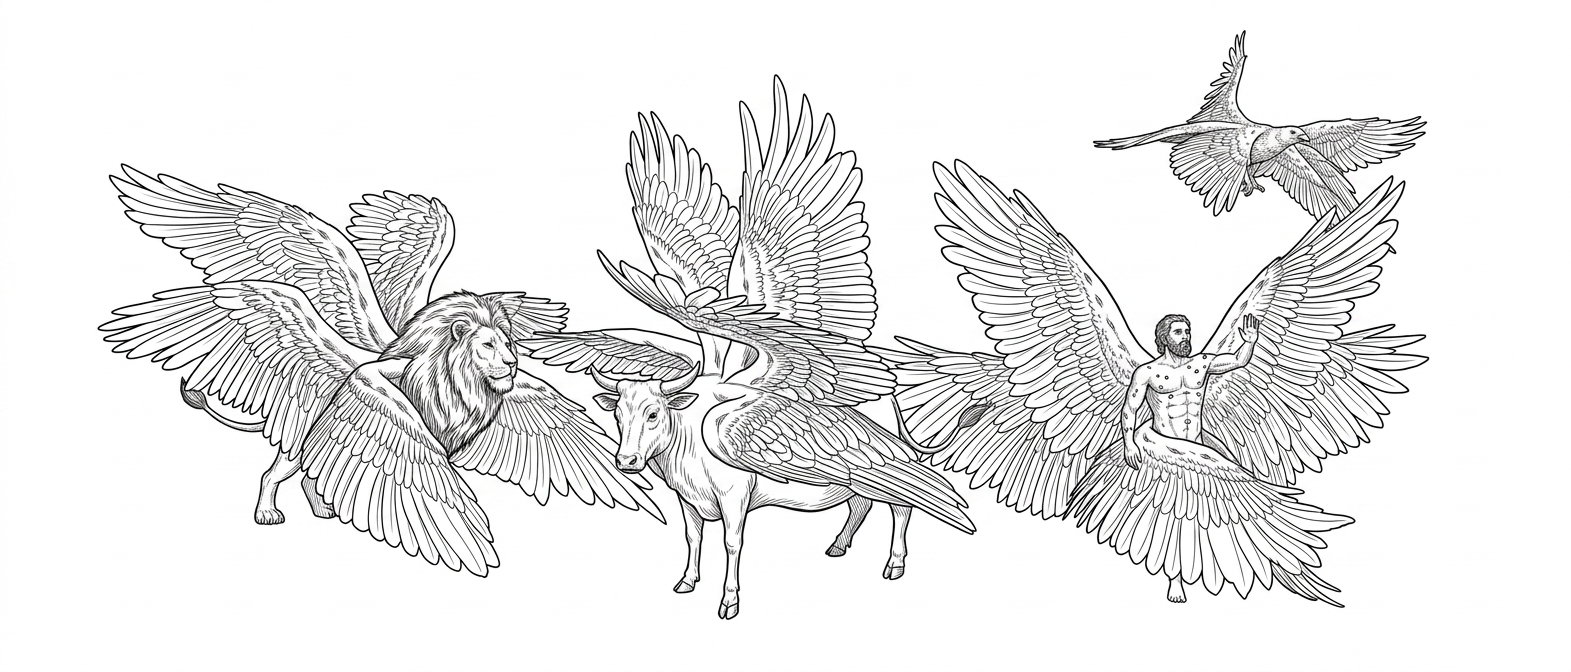
\includegraphics[
    width=1\textwidth, 
    trim=100 50 100 30, 
    clip]{images/four_living_creatures.jpg}
\end{figure}

\begin{ReaderQuestion}
表\ref{table:rev3_comp}對照此三處的異象。請圈出它們相似之處。
\end{ReaderQuestion}

這裡四個大有能力的活物，地上已經沒有任何生物如同他們。
四活物全身上下都有眼睛，牠們觀看並守望上帝所創造的一切，象徵上帝全知與無所不察。\footnote{MacArthur, J. (2007). Osborne, G. R. (2002).}
啟示錄 4:7 與以西結書1:10 是對照的。見表\ref{tab:four-living-creatures-zh}。
{
\renewcommand{\arraystretch}{1}
\small
\begin{longtable}{p{2.6cm} p{2.6cm}}
\caption{四活物：啟示錄4:7與以西結書1:10}
\label{tab:four-living-creatures-zh} \\
\hline
啟示錄 4:7 &
以西結書1:10 \\
\hline
像獅子 & 獅子臉 \\
像牛犢 & 牛臉 \\
像人 & 人臉 \\
像飛鷹 & 鷹臉 \\
\hline
\end{longtable}
}

\begin{ReaderQuestion}
四活物晝夜不住地宣告：「聖哉、聖哉、聖哉，主神是昔在、今在、以後永在的全能者。」上帝的聖潔、永恆與全能，對我們今天的敬拜生活有什麼意義？
\end{ReaderQuestion}

\section{頌讚創造萬有的主}

\begin{ScriptureBox2}{劃出二十四位長老所做的三件事，並圈出他們說上帝配得的原因。}

\item[4:10] 那二十四位長老、就俯伏在坐寶座的面前、敬拜那活到永永遠遠的、又把他們的冠冕放在寶座前、說、

\item[4:11] 我們的主、我們的　神、你是配得榮耀尊貴權柄的．因為你創造了萬物、並且萬物是因你的旨意被創造而有的。

\end{ScriptureBox2}

舊約聖經中，尤其是詩篇，有豐富的頌讚是關於神的創造的。我們在讀啟示錄時，更應該將舊約相關的經文放在一起，形成一個更豐富的認識。
這裡4:11的創造主題可以同時使人想到創世記 1 章、詩篇 33 篇、95 篇及 96 篇。\footnote{Bauckham, R. (1993).}
創世記1章說起初神創造天地，並創造人類。 
詩篇 33 篇說耶和華說有就有．命立就立。
詩篇 95:3–7讚美耶和華是大君王；海洋、山嶺與地的深處都屬於祂，因祂創造萬有，百姓當敬拜祂。
詩篇 96:4–5讚美耶和華超越列國的神明，因祂創造諸天，配受列國敬拜。
上帝不僅是創造萬物的主，也是整個受造界的君王。二十四位長老\idx{02}{二十四位長老}將冠冕放在寶座\idx{20}{寶座}前。一切受造者的尊榮與權柄都源於上帝，最終也當歸於祂。

\begin{ReaderQuestion}
創世記 1 章、詩篇 33、95、96 篇，都從不同角度頌讚上帝的創造。當我們真正認識上帝是萬物的創造主，這會如何改變我們看待自己的生命、工作，以及受造世界的態度？
\end{ReaderQuestion}

\section{沒有配展開書卷的}

\begin{ScriptureBox2}{圈出每一個「配」字，並劃出三個找不到任何人的地方。約翰為什麼大哭？}

\item[5:1] 我看見坐寶座的右手中有書卷、裡外都寫著字、用七印封嚴了。

\item[5:2] 我又看見一位大力的天使、大聲宣傳說、有誰配展開那書卷、揭開那七印呢。

\item[5:3] 在天上、地上、地底下、沒有能展開能觀看那書卷的。

\item[5:4] 因為沒有配展開、配觀看那書卷的、我就大哭。

\end{ScriptureBox2}
\begin{figure}[htbp]
    \centering
    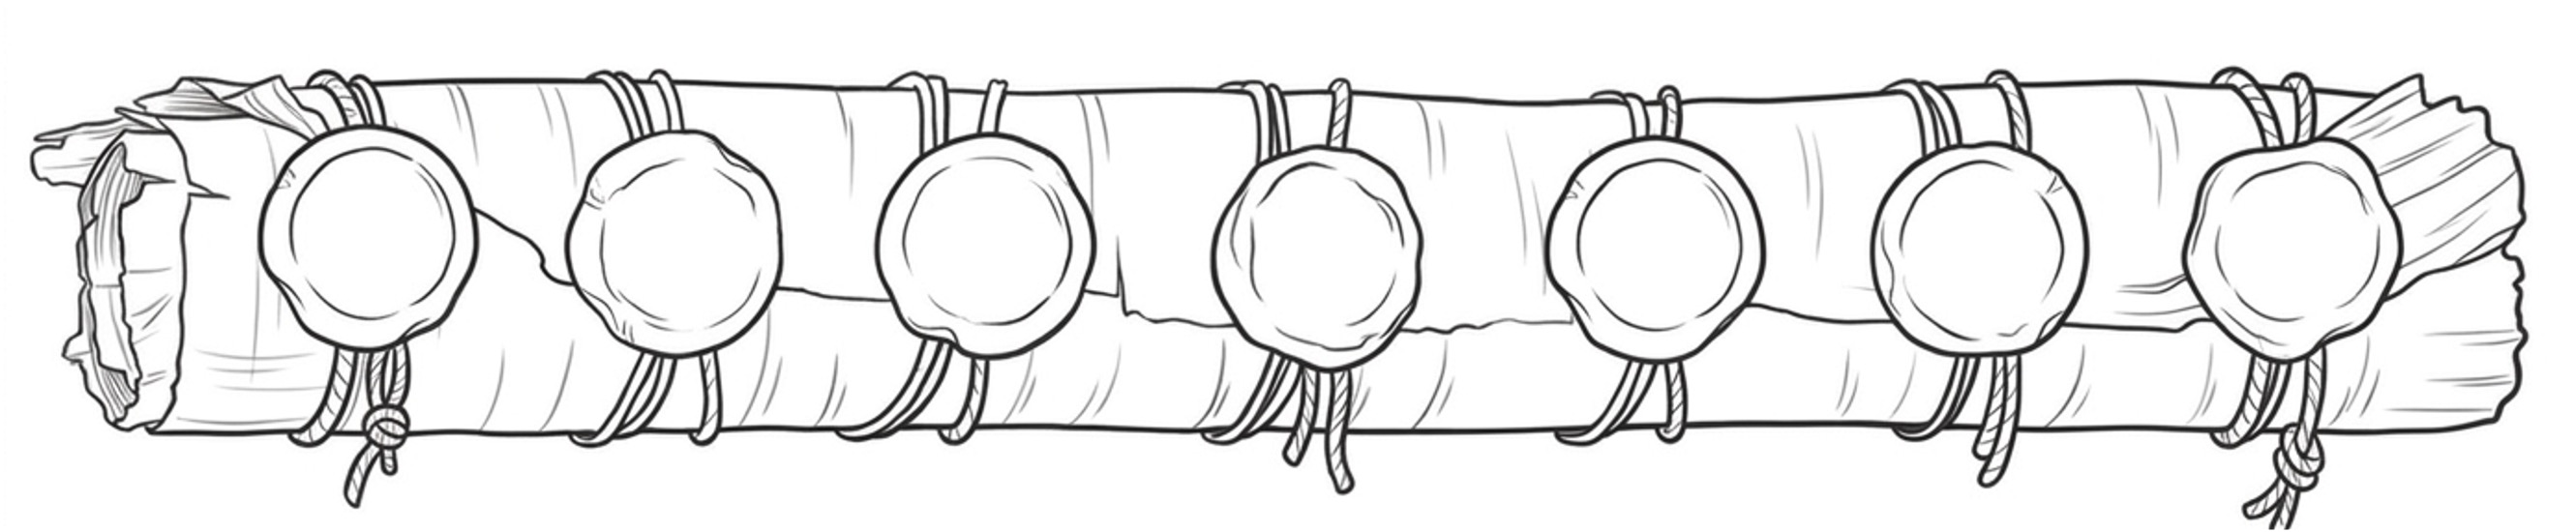
\includegraphics[
    width=1\textwidth, 
    trim=0 0 0 0, 
    clip]{images/scroll_light.jpg}
\end{figure}

歷史掌握在神的手中，並且藉著書卷\idx{10}{書卷}頒給出來。然而，誰配得揭開書卷，使神的旨意進入實現？受造界中竟然無人配得。這使的約翰大哭。
這不僅是因為他無法看見書卷的內容，更是因為若無人配得揭開書卷，上帝的救贖\idx{11}{救贖}與審判\idx{15}{審判}計畫便無法由任何受造者展開。\footnote{這讓我們想到以西結書也有書卷，也都內外寫著字。可是那個書卷是展開的，不是這裡的書卷。以西結書2:9-10：「我觀看、見有一隻手向我伸出來、手中有一書卷。
他將書卷在我面前展開、內外都寫著字、其上所寫的有哀號、歎息、悲痛的話。」}

為什麼是古代的書卷？如果讀者是現代的人或是未來的人，那就不是書卷了。當然，約翰不是在描寫未來的出版科技，而是在使用他所處時代可理解的啟示媒介。
古代以蒲草紙或其他材料製成卷軸。因此，約翰看見的不是一本現代裝訂的書，更不是一份現代的數位文件。


\section{被殺的羔羊才是真正的得勝君王}

\begin{ScriptureBox2}

\item[5:5] 長老中有一位對我說、不要哭．看哪、猶大支派中的獅子、大衛的根、他已得勝、能以展開那書卷、揭開那七印。

\item[5:6] 我又看見寶座與四活物並長老之中、有羔羊站立、像是被殺過的、有七角七眼、就是　神的七靈、奉差遣往普天下去的。

\item[5:7] 這羔羊前來、從坐寶座的右手裡拿了書卷。

\end{ScriptureBox2}
這裡又讓我們看見本書第一章所說的耶穌的形象：祂既是曾經受苦、被殺的主，也是從死裡復活、滿有榮耀\idx{14}{榮耀}與權柄的主。

羔羊\idx{10}{羔羊}使我們想到祂的受死、犧牲與救贖\idx{11}{救贖}；猶大的獅子\idx{12}{猶大的獅子}則使我們想到祂的君王身分、權柄與得勝\idx{11}{得勝}。猶大的獅子，竟以被殺羔羊的形象出現。
基督藉著祂的受死與復活，成就救贖，並顯明君王的權柄。

接著，約翰看見羔羊有「七角七眼」。七眼就是上帝的七靈\idx{02}{七靈}，奉差遣往普天下去。
在舊約中，「角」常用來象徵力量、能力與王權。所以這裡說明基督的權柄與聖靈的工作。

\section{羔羊以自己的血買贖萬民}

\begin{ScriptureBox2}{圈出羔羊配得的原因，並劃出祂為祂的子民所做的事。將此與4:11中上帝配得的原因比較。}

\item[5:8] 他既拿了書卷、四活物和二十四位長老、就俯伏在羔羊面前、各拿著琴、和盛滿了香的金爐．這香就是眾聖徒的祈禱。

\item[5:9] 他們唱新歌、說、你配拿書卷、配揭開七印．因為你曾被殺、用自己的血從各族各方、各民各國中買了人來、叫他們歸於　神、

\item[5:10] 又叫他們成為國民、作祭司、歸於　神．在地上執掌王權。

\end{ScriptureBox2}

羔羊\idx{10}{羔羊}藉著自己的血買贖萬民，使他們歸於上帝。
這救贖\idx{11}{救贖}的歌是蒙恩的罪人能唱的。他們的歌聲中，唱出神對人奇異的恩典\idx{10}{恩典}，唱出人生命的改變，最後在神的榮耀\idx{14}{榮耀}裡。
祂不僅赦免我們的罪，更賜給我們新的身分，使我們成為屬上帝的國度和祭司。從前遠離上帝的人，如今得以親近祂；從前不配敬拜的人，如今竟能與天上的敬拜者一同頌讚羔羊！

\section{從約翰的哭泣到全宇宙的敬拜}

\begin{ScriptureBox2}{圈出每一個參與敬拜的群體。}

\item[5:11] 我又看見、且聽見、寶座與活物並長老的周圍、有許多天使的聲音．他們的數目有千千萬萬．

\item[5:12] 大聲說、曾被殺的羔羊、是配得權柄、豐富、智慧、能力、尊貴、榮耀、頌讚的。

\item[5:13] 我又聽見、在天上、地上、地底下、滄海裡、和天地間一切所有被造之物、都說、但願頌讚、尊貴、榮耀、權勢、都歸給坐寶座的和羔羊、直到永永遠遠。

\item[5:14] 四活物就說、阿們。眾長老也俯伏敬拜。

\end{ScriptureBox2}

%\begin{figure}[htbp]
%    \centering
%    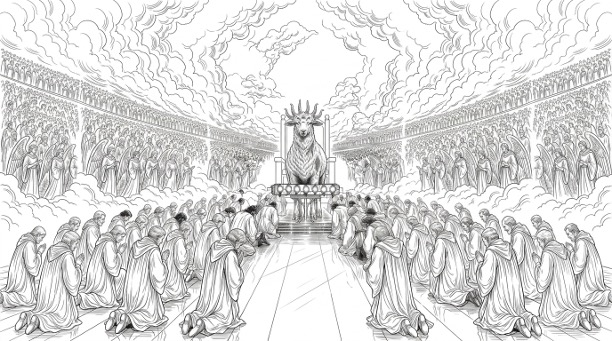
\includegraphics[
%    width=1\textwidth, 
%    trim=0 0 0 0, 
%    clip]{images/lamb_get_scroll2.jpg}
%\end{figure}

這真是偉大的頌讚。敬拜的範圍從千千萬萬的天使，擴展到天上、地上、地底下、滄海裡一切被造之物。萬有都將頌讚、尊貴、榮耀\idx{14}{榮耀}、權勢歸給坐寶座\idx{20}{寶座}的和羔羊\idx{10}{羔羊}，直到永永遠遠。
第四章呈現上帝因創造萬有而配得的敬拜，第五章則呈現羔羊因完成救贖\idx{11}{救贖}而配得的敬拜。
見表\ref{tab:rev4-5-worship-zh} 。

{
\renewcommand{\arraystretch}{1}
\small
\begin{longtable}{p{1cm} p{4cm} p{4cm}}
\caption{啟示錄4--5章的兩首頌讚：創造與救贖}
\label{tab:rev4-5-worship-zh} \\
\hline
敬拜 &
第四章：創造的頌讚 &
第五章：救贖的頌讚 \\
\hline
對象 &
坐寶座的主 &
坐寶座的主與羔羊\\

原因 &
上帝創造了萬物 &
羔羊曾被殺，以自己的血買贖萬民 \\

內容 &
榮耀、尊貴、權柄、創造萬有 &
權柄、豐富、智慧、能力、尊貴、榮耀、頌讚 \\

群體 &
四活物\idx{05}{四活物}、二十四位長老\idx{02}{二十四位長老} &
四活物、二十四位長老、千千萬萬天使，一切被造之物 \\

信息 &
萬有因上帝的旨意而被創造 &
萬民因羔羊的血蒙救贖，歸於上帝 \\
\hline
\end{longtable}
}

\begin{ReaderQuestion}
在你自己的生命中，你可以為什麼事讚美上帝是創造主？又可以為什麼事感謝羔羊是你的救贖主？
\end{ReaderQuestion}

創造與救贖在此交會：那位曾被殺、如今仍然活著的羔羊，與坐在寶座上的上帝一同接受萬有永遠的敬拜。願我們日日敬拜讚美祂創造的大能，讚美的言詞，如海洋般澎湃。願我們日日稱頌祂救贖的恩典\idx{10}{恩典}，感恩的聲音，如江河般奔流，永不止息。
